\Chapter{Processz ütemezés}
\label{ch:scheduling}

\Section{Az ütemezési probléma}

% https://users.iit.uni-miskolc.hu/~vinczed/ldapauth/osbsc2019/Operacios-rendszerek-jegyzet.pdf

Minden operációs rendszer hatékonysága arányos azzal a képességével, amely a processzek igazságosnak tekinthető (\textit{fair}) ütemezését végzi. A processz ütemező, a kernel központi eleme, ő az aki eldönti, hogy mikor és mennyi időre birtokolhatja egy folyamat a processzort. Ideális esetben, a processzeknek időszeletekre van szükségük a futáshoz, az ütemezőknek lényegében a processzor időszeleteit kell tisztességesen felosztaniuk a folyamatok között \cite{tanenbaum1999operacios}.

Egy ütemező algoritmusnak többek között a következőkben felsorolt kritériumokat kell teljesíteniük.
\begin{itemize}
	\item Pártatlanság: minden folyamat (processz, taszk, job) korrekt módon (nem feltétlenül egyenrangúan) kapjon CPU-t.
	\item Hatékonyság: a CPU lehetőleg a legnagyobb százalékban legyen kihasználva a hasznos számításokra nézve.
	\item Válaszidő: az interaktív felhasználóknak a válaszidőt minimalizálják, (ne vesszék el türelmüket, hiszen a "vakon" nyomogatott gombok tovább lassíthatnak).
	\item Fordulási idő (\textit{turnaround time}): a kötegelt munkák (job) fordulási idejét minimalizálni kell.
	\item Teljesítmény: az időegységre eső job-feldolgozás, interaktív munka maximalizálása.
(Lássuk be, ez különbözik a fent említett hatékonyságtól.)
\end{itemize}
Láthatók bizonyos ellentmondások a kritériumok között. A válaszidő minimalizálása eredményezheti a fordulási idő növekedését!
A számításigényes munkák korlátozás nélküli
előnyben részesítése javítja a hatékonyságot, de nem biztosítja a korrektséget, és az összevont
teljesítmény is csorbulhat.
Jelenleg a Linux kernel 5.8.x verziójában, a normál processzek ütemezését a CFS (\textit{Completely Fair Scheduler}) ütemezési osztály végzi \cite{wong2008towards}.

\Section{Elterjedt ütemezési stratégiák}

\SubSection{Lineáris idejű ütemezés}

Az $\mathcal{O}(n)$ ütemező, amelyet a Linux kernelben használtak 2.4 és 2.6 verziók között. A müködési elve egyszerűnek mondható, mivel végigiterál az összes futásra kész állapotú processzen, és megválasztja a legmagasabb prioritási értékkel rendelkezőt.
Ez egy $\mathcal{O}(n)$ műveletigényű algoritmus volt, ahol az $n$ a futtatható processzek számát jelölte. Emiatt nagy processzámnál nem volt elég hatékony és a valós idejű processzek így kiszámíthatlanok lettek \cite{programmersought}.
Egy futási sort (\textit{runqueue}-t) használt, hogyha a processzek száma kevesebb volt, mint a processzormagok száma. A maradék processzor egy "tétlen" állapotba került. Emiatt ez az ütemező nem volt túl hatékony erőforrás kihasználásban sem.

\SubSection{Konstans idejű ütemezés}

Az $\mathcal{O}(n)$ ütemező különféle problémái miatt, leváltotta az $\mathcal{O}(1)$ ütemező, amit a Linux kernel 2.6 verziójától, 2.6.22 verzióig használták. 
Konstans idő alatt választott következő processzt futásra, emiatt nagy processz szám mellett is használható volt.
A folyamatokat, két részre osztotta: Real-time illetve normál processzekre. A valós idejű processzek 0-99-ig kapnak prioritási szinteket, amíg a normál processzek (Batch vagy interactive) 100-139-ig. Itt a 100-as prioritás jelöli a legfontosabb processzt, amíg a 139 a legkevésbé fontosat. Normál processzekhez egy alapértelmezett 120-as statikus prioritást rendeltek \cite{wong2008fairness, rebeiro2020scheduling}.

Processzoronként, két listát tart nyilván, amiben tárolódnak a futásra kész processzek: \textit{Active run queue}, \textit{Expired run queue} (\ref{fig:activeExpiredRunqueue}. ábra).

\begin{figure}[h]
\centering
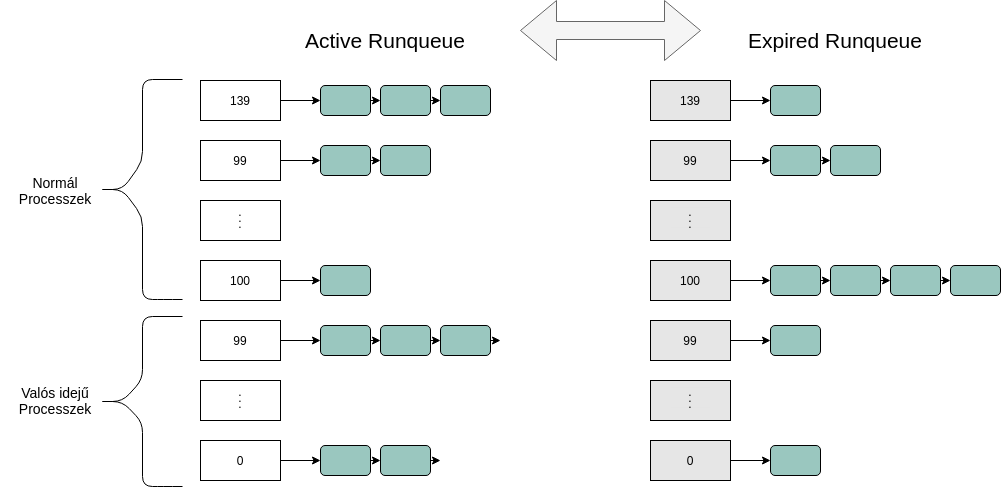
\includegraphics[width=\textwidth]{images/activeExpiredRunqueue.png}
\caption{Active and Expired Run queues}
\label{fig:activeExpiredRunqueue}
\end{figure}

Mindig az aktív listából választja ki a legfontosabb processzt futásra. Miután futott egy időszeletnyit, ez a processz, átkerül az expired run queue-ba, egy új dinamikusan számolt prioritással.
Emiatt, ahogy haladunk előre az időben az \textit{Active run queue}-ból folyamatosan fogynak el a processzek.  Amikor az \textit{Active run queue} végzett a processzekkel, a két lista felcserélődik és folyatatódik a végrehajtás az új listával.
Annak érdekében, hogy meg lehessen különböztetni a batch és az interactive processzeket, egy úgynevezett "bonus" valtozót tartunk nyilván, ami a dinamikus prioritás számításnál fog előkerülni. Ennek az értéke 0 és 10 között mozgó egész érték \cite{aas2005understanding}.
\begin{cpp}
dynamic priority = MAX(100, MIN(static priority - bonus + 5, 139))
\end{cpp}
Amikor a bonus változó értéke kisebb mint 5, az arra utal, hogy kevesebb interakciót fog végezni a felhasználóval, így több CPU lázas szakasza lesz a processznek élete során. Ilyenek tipikusan a batch processzek.
Ha a bonus változó értéke nagyobb mint 5 lesz, valószínűleg a processz élete során sok interakciót fog végezni a felhasználóval. A magas bonus változó érték tehát az interaktív processzekre jellemző. Tekintsük át ezen két, jellemző típust!
\begin{itemize}
\item \textit{Batch Process}: Nem igényelnek felhasználóval történő interakciót, általában a háttérben futnak. Ezeknek a processzeknek nincs szükségük arra, hogy reszponzívak legyenek, tipikusan ilyenek a programozási nyelvek fordítói, adatbázis motorok és tudományos számítások.
\item \textit{Interactive Process}: Folytonos interakciót igényelnek a felhasználóval, az életidejük nagy részét gomb leütésekre és egér mozdulatokra történő várakozással töltik.
Amikor az input beérkezik, gyorsan reagálniuk kell, ellenkező esetben a felhasználó lassúnak fogja találni a rendszert (amit természetesen ezt el szeretnénk kerülni).
Az interactive processzek általában nem fejezik be az időszeletüket amit kapnak, ezért nekik nagyobb időszeletet kell biztosítani, mivel kisebb részeket töltenek CPU idővel (amikor folyamatosan instrukciókat hajtanak végre) és az idő nagyobb részében I/O ra várakoznak.
\end{itemize}

% Az interaktív processzek általában, kisebb részeket töltenek CPU idővel(amikor folyamatosan instrukciókat hajtanak végre) és az idő nagyobb részében I/O ra várakoznak.
% Annak érdekében hogy ezeket a kis CPU-s sorozatokat egyben befejezzék, nagy időszeletet próbál biztosítani számukra, ez az ütemező.
% Ez itt a következő {cpp}-s részben is látszik, hogy a 120-as prioritásnál kisebb értékkel rendelkező processzeket(akik nagyon fontosak) nevezzük interaktívnak és nekik az időszeletüket, egy nagyobb szorzóval látjuk el. Ezt az időszeletet valószínűleg nem fogják kihasználni, csak biztosítani szeretnénk számukra hogy a CPUs életidejüket teljesen befejezzék és utána, önmaguktól úgyis lemondanak majd a processzorról. 

Az időszelet meghatározása úgy történik, hogy amelyik processz kevesebb mint 120-as prioritással rendelkezik, nagyobb időszeletet kap, 120-nál nagyobb prioritású processzek pedig kevesebbet. A számítás Python forráskód formájában a következőképpen szemléltethető
\begin{python}
if priority < 120:
    time_slice = (140 - priority) * 20
else
    time_slice = (140 - priority) * 5
\end{python}
ahol az időszelet (\texttt{time\_slice}) értéke ezredmásodpercben van megadva \cite{rebeiro2020scheduling, wong2008fairness}.

%TODO referencia: https://doc.opensuse.org/documentation/leap/tuning/html/book-sle-tuning/cha-tuning-taskscheduler.html#sec-tuning-taskscheduler-cfs
%TODO referencia: https://elixir.bootlin.com/linux/v5.8.5/source/kernel/sched/fair.c
%TODO referencia könyvből: Linux Kernel Development 3rd Edition 51.oldal

\Section{A linux ütemező felépítése}

A GNU/Linux operációs rendszer elsődlegesen asztali gépekhez lett tervezve, ennek ellenére hamar multi-dimenziós operációs rendszerré nőtte ki magát, széles körben használják beágyazott rendszereken, szervereken, mainframe-eken és szuperszámítógépeken is. Különböző platformok is befogadták, mint például valós idejű rendszerek, SMP, virtualizáció. Az ilyen változatos platformok miatt, alakultak ki a típusai a processzeknek. Egy asztali rendszeren, többnyire magas interaktivitású processzeket kell ütemezni, amik I/O igényesek, a valós idejű rendszereken pedig inkább  determinisztikus processzek a jellemzőek. A különböző típusú processzeket, egymástól eltérő heurisztikus módszerekkel ütemezhetjük fair módon.

\SubSection{Ütemezési osztályok}

A Linux ütemező moduláris, emiatt lehetővé teszi, hogy különböző algoritmusok ütemezzenek különböző típusú processzeket. Ezt a modularitást, ütemező osztályoknak nevezzük. Belső kialakitása igen ügyesen kezeli a különböző processz típusokat két rétegű modell felhasználásával (\ref{fig:genericScheduler}. ábra).
\begin{itemize}
\item Az első réteg egy általános ütemező (\textit{Generic Scheduler}), ami absztrakt műveleteket határoz meg. Ez egy belépési függvény az ütemező számára.
\item A második rétegben maguk az ütemező osztályok helyezkednek el (\textit{Scheduler Classes}), ami a tényleges ütemezési műveleteket tartalmazza. Itt történik a különböző  processz osztályok ütemezése.
\end{itemize} 

\begin{figure}[h]
\centering
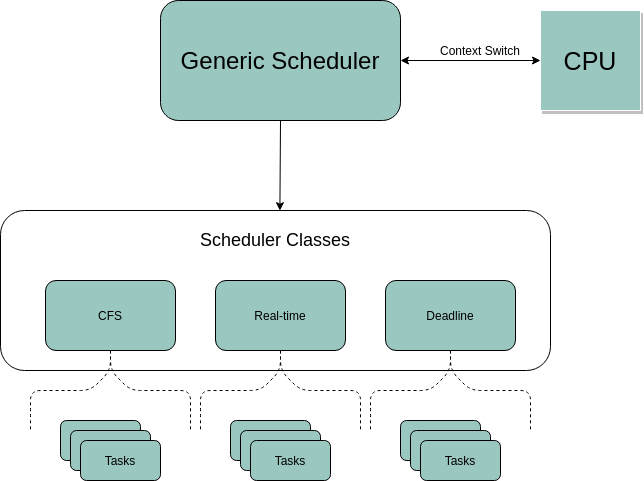
\includegraphics[width=\textwidth]{images/genericScheduler.png}
\caption{Az általános ütemező és a specializált ütemező osztályok.}
\label{fig:genericScheduler}
\end{figure}

Ez a modell lehetővé teszi, hogy a \textit{Generic Scheduler} elvont maradjon minden ütemező osztály megvalósítási részleteitől. Így a normál processzek ütemezéséért, az egyik ütemező osztály felel, amíg determinisztikus végrehajtást igénylő processzekért, mint a valós idejű folyamatok, egy másik osztály. Ez az architechtúra lehetővé teszi azt is hogy, akár új ütemező osztályt vezessünk be.

A \textit{Generic Scheduler} egy absztrakt interfészt definiál a (\texttt{/kernel/sched/sched.h}-ban lévő) \texttt{sched\_class} struktúrán keresztül. A működés megértéséhez egyszerűbb és pontosabb közvetlenül az implementációt tekinteni.

%TODO referencia: https://elixir.bootlin.com/linux/v5.8.5/source/kernel/sched/sched.h#L1743
\begin{cpp}
struct sched_class {
	const struct sched_class *next;

#ifdef CONFIG_UCLAMP_TASK
	int uclamp_enabled;
#endif

	void (*enqueue_task)
		(struct rq *rq, struct task_struct *p, int flags);
	void (*dequeue_task)
		(struct rq *rq, struct task_struct *p, int flags);
	void (*yield_task)   (struct rq *rq);
	bool (*yield_to_task)
		(struct rq *rq, struct task_struct *p, bool preempt);

	void (*check_preempt_curr)
		(struct rq *rq, struct task_struct *p, int flags);

	struct task_struct *(*pick_next_task)(struct rq *rq);

	void (*put_prev_task)(struct rq *rq, struct task_struct *p);
	void (*set_next_task)
		(struct rq *rq, struct task_struct *p, bool first);

#ifdef CONFIG_SMP
	int (*balance)
	  (struct rq *rq, struct task_struct *prev, struct rq_flags *rf);
	int  (*select_task_rq)
	  (struct task_struct *p, int task_cpu, int sd_flag, int flags);
	void (*migrate_task_rq)(struct task_struct *p, int new_cpu);

	void (*task_woken)(struct rq *this_rq, struct task_struct *task);

	void (*set_cpus_allowed)(struct task_struct *p,
				 const struct cpumask *newmask);

	void (*rq_online)(struct rq *rq);
	void (*rq_offline)(struct rq *rq);
#endif

	void (*task_tick)
		(struct rq *rq, struct task_struct *p, int queued);
	void (*task_fork)(struct task_struct *p);
	void (*task_dead)(struct task_struct *p);

	/*
	 * The switched_from() call is allowed to drop rq->lock, 
	 * therefore we
	 * cannot assume the switched_from/switched_to 
	 * pair is serliazed by
	 * rq->lock. They are however serialized by p->pi_lock.
	 */
	void (*switched_from)
		(struct rq *this_rq, struct task_struct *task);
	void (*switched_to) 
		(struct rq *this_rq, struct task_struct *task);
	void (*prio_changed)
		(struct rq *this_rq, struct task_struct *task,
			      int oldprio);

	unsigned int (*get_rr_interval)(struct rq *rq,
					struct task_struct *task);

	void (*update_curr)(struct rq *rq);

#define TASK_SET_GROUP		0
#define TASK_MOVE_GROUP		1

#ifdef CONFIG_FAIR_GROUP_SCHED
	void (*task_change_group)(struct task_struct *p, int type);
#endif
};

\end{cpp}
 
Minden ütemező osztálynak prioritása van. 
Az általános ütemező, végigiterál az ütemező osztályokon és azt a legnagyobb prioritással rendelkező osztályt fogja választani, amiben található futtatható processz. A megválasztott ütemezési osztály fogja eldönteni, hogy melyik processz kerülhet végrehajtásra.

A kernel 5.8.x verziójában, három ütemezési osztály található, név szerint: 
\begin{itemize}
	 \item Completely Fair Scheduler class,
	 \item Real-time class,
	 \item Deadline class.
\end{itemize}
A következő kódrészletek megmutatják, hogy az osztályok külön-külön hogyan definálják a \texttt{sched\_class} absztrakt struktúrát.

%TODO referencia: https://elixir.bootlin.com/linux/v5.8.5/source/kernel/sched/fair.c#L11126
Completely Fair Scheduler ütemezési osztályhoz tartozó fontosabb mezők az alábbiak (\texttt{/kernel/sched/fair.c}):

\begin{cpp}
const struct sched_class fair_sched_class = {
	.next			= &idle_sched_class,
	.enqueue_task		= enqueue_task_fair,
	.dequeue_task		= dequeue_task_fair,
	.yield_task		= yield_task_fair,
	.yield_to_task		= yield_to_task_fair,

	.check_preempt_curr	= check_preempt_wakeup,

	.pick_next_task		= __pick_next_task_fair,
	.put_prev_task		= put_prev_task_fair,
	.set_next_task          = set_next_task_fair,
...
};
\end{cpp}

%TODO referencia: https://elixir.bootlin.com/linux/v5.8.5/source/kernel/sched/rt.c#L24321
A Real-time Scheduler ütemezési osztály esetében (\texttt{/kernel/sched/rt.c}):

\begin{cpp}
const struct sched_class rt_sched_class = {
	.next			= &fair_sched_class,
	.enqueue_task		= enqueue_task_rt,
	.dequeue_task		= dequeue_task_rt,
	.yield_task		= yield_task_rt,

	.check_preempt_curr	= check_preempt_curr_rt,

	.pick_next_task		= pick_next_task_rt,
	.put_prev_task		= put_prev_task_rt,
	.set_next_task          = set_next_task_rt,
...
};
\end{cpp}

%TODO referencia: https://elixir.bootlin.com/linux/v5.8.5/source/kernel/sched/deadline.c#L2433
A Deadline Scheduler esetén (\texttt{/kernel/sched/deadline.c}):

\begin{cpp}
const struct sched_class dl_sched_class = {
	.next			= &rt_sched_class,
	.enqueue_task		= enqueue_task_dl,
	.dequeue_task		= dequeue_task_dl,
	.yield_task		= yield_task_dl,

	.check_preempt_curr	= check_preempt_curr_dl,

	.pick_next_task		= pick_next_task_dl,
	.put_prev_task		= put_prev_task_dl,
	.set_next_task		= set_next_task_dl,
...
};
\end{cpp}

%referencia: https://www.kernel.org/doc/html/latest/scheduler/sched-design-CFS.html

\SubSection{Ütemezési politikák}

A CFS osztály három ütemezési politikát (\textit{Scheduling policy}-t) implementál.
\begin{itemize}	
    \item SCHED\_OTHER (tradicionálisan  SCHED\_NORMAL) - Alapértelmezett ütemezési algoritmus, amit a normál processzek nagytöbbsége is használ.

    \item SCHED\_BATCH - Közel sem hajt végre olyan sok preempciót mint az átlagos taszkok, ezáltal lehetővé téve azt, hogy a taszkok tovább fussanak, de ennek az ára az interaktivitás csökkenése.
        
	  \item \texttt{SCHED\_IDLE} - Ezt az ütemezési politikát, kis intenzitású processzek esetén használják. Ezzel még a \texttt{nice} $+19$-től kisebb prioritást szabhatunk a processzünknek.
\end{itemize}
A valós idejű ütemezési osztály implementálja a \texttt{SCHED\_FIFO} és \texttt{SCHED\_RR} politikákat, ezek a POSIX által lettek meghatározva.
\begin{itemize}
	\item SCHED\_FIFO - Időkritikus, valós idejű processzek ütemezésénél használják. A nevében is benne van, FIFO jellegű azaz First-In First-Out, az elsőnek érkezett processz kerül először kiszolgálásra. 
	\item SCHED\_RR - SCHED\_FIFO-hoz hasonló, szintén valós idejű processzekhez használják. A \textit{Round Robin} ütemezési algoritmust használja.
\end{itemize}
% TODO: Tényleg használják "Kerge Rigó" néven? :)
% TODO:-Nem igazán használják és nem is szokták fordítani magyarra.
% Ennek ellenére ez a fordítás megragadt bennem és amikor ezt a részt írtam elfelejtettem hogy nem kellene így írnom, viszont most kijavítottam a normális változatra.
% TODO: Dr. Vadász Dénes Operációs rendszerek jegyzetében olvastam ezt először, 
% "2.4.6. Round-Robin scheduling
% Egyszerű, korrekt, széleskörben használható, könnyen megvalósítható, elég régi algoritmus
% ez. Nem szokták magyarra fordítani az elnevezést: elég furcsa lenne a kerge-rigó név!"

A SCHED\_DEADLINE politika, a \texttt{sched\_dl} ütemezési osztályban található. Az EDF (\textit{Earliest Deadline First}) ütemezési algoritmus az implementációja.

\SubSection{Runqueues}

Hagyományosan a \textit{runqueue} az az adatstruktúra, ami tárolja az összes processzt, akik a CPU-ért versenyeznek.
Minden processzor maghoz, külön \textit{runqueue} tartozik. 
A \textit{Generic Scheduler} réteg egy absztrakt \textit{runqueue}-t implementál, olyan elemekkel, amik egy \textit{runqueue} interfésznek felelnek meg.
Ez a struktúra ki lett bővítve néhány pointerrel, amik a különböző osztályok futási soraikra mutatnak. Ez azt jelenti, hogy a különböző ütemezési osztályok futási soraik, mind bele vannak ágyazva a fő \textit{runqueue} struktúrába. Ezáltal minden ütemező osztálynak lehetősége van megválasztani, a saját \textit{runqueue} adat struktúráját.

\SubSection{Processz Prioritási szintek és azok módosítása}

Annak az eldöntése, hogy melyik processz kerül legközelebb végrehajtásra, függ a prioritástól. Minden processz el van látva egy prioritás értékkel, ami lehet dinamikus prioritás vagy statikus prioritás.

Dinamikus prioritásnak nevezzük azt, amit a kernel normál folyamatoknál alkalmaz. Ehhez az értékhez figyelembe veszi a processz nice értékét, az elmúlt időben megfigyelt tevékenységét (CPU vagy I/O lázas processz), és hogy mennyi időt töltött várakozással, illetve  végrehajtással.
A normál processzekhez alapértelmezett prioritását meg tudjuk változtatni a \texttt{nice}, illetve a \texttt{renice} paranccsal.
\begin{python}
$ nice -n N ./a.out 
\end{python}%$
Ebben az \texttt{N} értéke +19 és -20 között mozoghat.
Nagyobb \textit{nice} érték azt jelzi, hogy mennyire vagyunk "nagylelkűek" a többi programhoz, azáltal, hogy őket előre engedjük.

A processzek \textit{nice} értékeiket lekérdezhetjük a \texttt{ps} programmal az alábbi formában.
\begin{python}
$ ps -Al
\end{python}%$

Statikus prioritást valós idejű processzeknél alkalmaznak. Ilyen prioritást felhasználó is adhat processznek. Ekkor a kernel nem módosíthatja dinamikusan az értéket.
A statikus prioritású processzek tehát elsőbbséget élveznek ütemezéskor.
Egy processz statikus prioritási értéke adott ütemezési politikákhoz mérten változhat. Ezeket a \texttt{chrt -m} paranccsal láthatjuk, például:
\begin{python}
$ chrt -m
SCHED_OTHER min/max priority	: 0/0
SCHED_FIFO min/max priority	: 1/99
SCHED_RR min/max priority	: 1/99
SCHED_BATCH min/max priority	: 0/0
SCHED_IDLE min/max priority	: 0/0
SCHED_DEADLINE min/max priority	: 0/0
\end{python}%$


A linux kernel szemszögéből, a processz prioritásokat skálázása 0-tól, 139-ig történik. A valós idejű processzek 0-tól 99-ig kapnak prioritást, amíg a normál folyamatok pedig 100-tól, 139-ig.


Normál processzek esetén 120-as a statikus prioritás, ezt az értéket módosíthatjuk, a \texttt{nice} illetve a \texttt{renice}-paranccsal, amelyből így a $[-20, +19]$ intervallum megválasztása is érthetővé válik.

A processzeknek lekérdezhetjük, illetve megváltoztathatjuk az ütemezési politikáikat szintén a \texttt{chrt} program segítségével. A példánkban a processzünk azonosítója (PID-je) 31475. Az ütemezési polika lekérdezéséhez tehát az alábbi parancsot adhatjuk ki.
\begin{python}
$ chrt -p 31475
pid 31475 current scheduling policy: SCHED_OTHER
pid 31475 current scheduling priority: 0
\end{python}%$

\noindent A processz ütemezési politikájának megváltozatása:
\begin{python}
$ chrt -rr -p 99 31475
$ chrt -p 31475
\texttt{pid} 31475 current scheduling policy: \texttt{SCHED_RR}
\texttt{pid} 31475 current scheduling priority: 99
\end{python}%$

Valós idejű (Real-time) processzek esetén, a prioritási szintjeik ellentétesek a normál processzekéhez képest. A legfontosabb prioritási szint a 99-es és a legkevésbé fontos pedig az 1-es \cite{redhat2019deadline}.

DeadLine processzek is ugyanilyen egyszerűen készíthetők a \texttt{chrt} programmal.
Itt viszont ki kell bővítenünk három paraméterrel a programunkat.
\begin{itemize}
\item Runtime: A feladatra kijelölt végrehajtási idő.
\item Deadline: A periódus megkezdése után milyen gyorsan kell elindítani a futási időt.
\item Period:  Milyen gyakran kerül végrehajtásra.
\end{itemize}

A kernel megköveteli, hogy a következők igazak legyenek:
\[
\text{RUNTIME} \leq \text{DEADLINE} \leq \text{PERIOD}.
\]
Bármelyik paraméter elhagyása az alábbiakat eredményezi.
\begin{itemize}
\item A futásidő elhagyása azt eredményezi hogy, futási időt a határidő értékére kell állítani.
\item A határidő elmulasztása azt eredményezi, hogy a határidőt a periódus értékére kell beállítani.
\item A periódus elmulasztása a periódust, a határidő értékére kell állítani.
\end{itemize}
\noindent Ezzel a három plusz paraméterrel, így néz ki a \texttt{chrt} program paraméterezése:
\begin{python} 
$ sudo chrt -d --sched-runtime 1ms --sched-deadline 5ms 
		--sched-period 5ms 0 ./test
\end{python}%$

% TODO: Itt érdemes a mértékegységet is megadni.

\SubSection{Completely Fair Scheduler}
\label{sec:cfs}

A \textit{Completely Fair Scheduler} váltotta le a korábbi $\mathcal{O}(1)$ ütemezőt a linux kernel 2.6.23 verzióban.
Az összes dinamikus prioritású folyamatot a CFS osztály kezeli. Általános célú Unix rendszerekben, normál processzekből fordul elő a legtöbb, ebből is következik, hogy a CFS ütemező osztály a legelfoglaltabb.
A CFS nem támaszkodik a hagyományos időszeletekre a processzor kiosztásakor, hanem inkább a virtuális futásidő (vruntime) fogalmát vezeti be.
A vruntime változó tárolja el a virtuális futás idejét egy processznek, ami igazából a tényleges futási idő normálizálva, a futtatható processzek darabszámával.

A virtual runtime mértékegysége a nanoszekundum ($10^{-9}$ másodperc).
A virtual runtime segítségével szeretnénk megközelíteni az ideális multitasking processzort, amit a CFS próbál modellezni. Egy egyszerű szabályt követ az algoritmus, ami pedig az, hogy mindig válassza a legkisebb vruntime-al rendelkező taszkot. A CFS egy piros-fekete fát használ, a listában lévő futtatható taskok kezelésére, hogy egyszerűen megtalálhassa a legkisebb vruntime-mal rendelkező taskot.
A piros-fekete fa, amelyet a Linux kernel esetében \texttt{rbtree}-nek hívnak, egy saját magát kiegyensúlyozó bináris fa.
A fában a csomópontok egy-egy futásra kész taszkot reprezentálnak. A taszkok elhelyezkedése a fában a virtuális futásidejükhöz mérten történik. 
A fa bal oldalában helyezkednek el a kisebb vruntime-mal rendelkező taszkok.
A balszélső csomópontban mindig az a taszk található, amelyik a legkevesebb a vruntime-mal rendelkezik.
\begin{figure}[h]
\centering
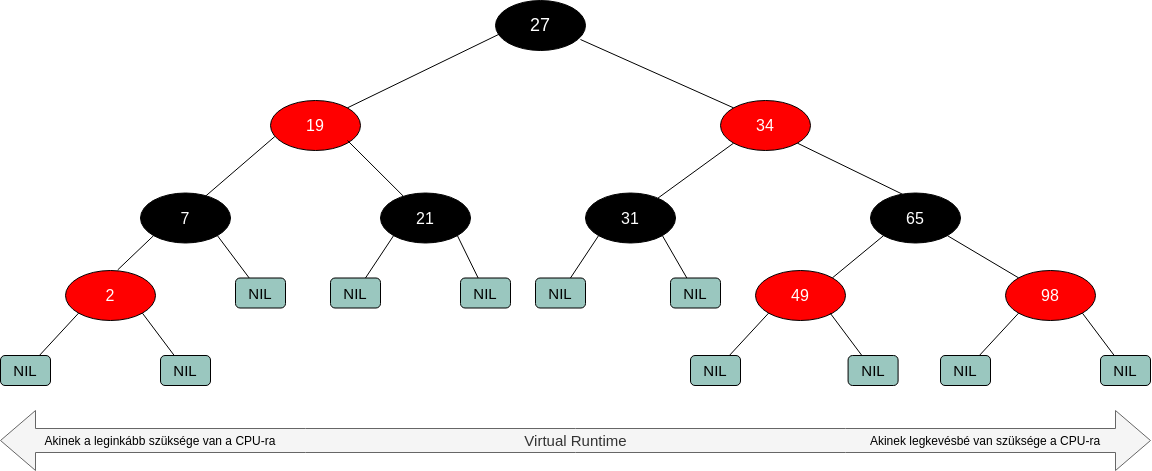
\includegraphics[width=\textwidth]{images/redBlackTree.png}
\caption{Piros fekete fa a processz prioritás értékekkel}
\label{fig:rb_tree}
\end{figure}

\noindent A piros-fekete fák önkiegyensúlyozók maradnak azáltal hogy, betartják az alábbi öt tulajdonságot.

\begin{enumerate}
	\item Egy csúcs vagy fekete vagy piros.
	\item A fa gyökere fekete.
	\item Egy piros csúcs mindkét leszármazottja fekete.
	\item Minden levél a fa gyökerével egyszínű. 
	\item Minden csúcsból a belőle leszármazó levelekbe vezető egyszerű utakon ugyanannyi fekete csúcsot érintünk.
\end{enumerate}

Amikor egy taszk futásra kész állapotba kerül, meghívódik a \texttt{enqueue\_task\_fair()}  függvény, ami hatására bekerül a piros-fekete fába. Amint a taszk kilépett ebből az állapotból, az ütemező \texttt{dequeue\_task\_fair()} segítségével eltávolítja a fából.
A következő kódrészletben látható hogy milyen függvényeket használ az ütemező a runqueue kezeléséhez.

\begin{cpp}
/*
 * All the scheduling class methods:
 */
const struct sched_class fair_sched_class = {
	.next			= &idle_sched_class,
	.enqueue_task		= enqueue_task_fair,
	.dequeue_task		= dequeue_task_fair,
	.yield_task		= yield_task_fair,
	.yield_to_task		= yield_to_task_fair,

	.check_preempt_curr	= check_preempt_wakeup,

	.pick_next_task		= __pick_next_task_fair,
	.put_prev_task		= put_prev_task_fair,
	.set_next_task          = set_next_task_fair,

#ifdef CONFIG_SMP
	.balance		= balance_fair,
	.select_task_rq		= select_task_rq_fair,
	.migrate_task_rq	= migrate_task_rq_fair,

	.rq_online		= rq_online_fair,
	.rq_offline		= rq_offline_fair,

	.task_dead		= task_dead_fair,
	.set_cpus_allowed	= set_cpus_allowed_common,
#endif

	.task_tick		= task_tick_fair,
	.task_fork		= task_fork_fair,

	.prio_changed		= prio_changed_fair,
	.switched_from		= switched_from_fair,
	.switched_to		= switched_to_fair,

	.get_rr_interval	= get_rr_interval_fair,

	.update_curr		= update_curr_fair,

#ifdef CONFIG_FAIR_GROUP_SCHED
	.task_change_group	= task_change_group_fair,
#endif

#ifdef CONFIG_UCLAMP_TASK
	.uclamp_enabled		= 1,
#endif
};
\end{cpp}

A \texttt{vruntime} váltózó értékének kiszámításához, a CFS nem csak a \texttt{nice} értéket használja fel hanem a process load weight változóját is. A \texttt{nice} értékben történő lépegetés egyesével felfelé, minusz 10\% CPU időszeletet fog eredményezni, és minden lépés lefelé pedig plusz 10\%-ot. 
A processz load weight változójának kiszámolásához a kernel fenttart egy tömböt amit \textit{sched\_prio\_to\_weight}-nek neveztek el. Itt megtalálható, hogy melyik \texttt{nice} értékhez, milyen súly érték tartozik.
%TODO referencia a forráskódból: https://elixir.bootlin.com/linux/v5.8.5/source/kernel/sched/core.c#L8182
\begin{cpp}
const int sched_prio_to_weight[40] = {
 /* -20 */     88761,     71755,     56483,     46273,     36291,
 /* -15 */     29154,     23254,     18705,     14949,     11916,
 /* -10 */      9548,      7620,      6100,      4904,      3906,
 /*  -5 */      3121,      2501,      1991,      1586,      1277,
 /*   0 */      1024,       820,       655,       526,       423,
 /*   5 */       335,       272,       215,       172,       137,
 /*  10 */       110,        87,        70,        56,        45,
 /*  15 */        36,        29,        23,        18,        15,
};
\end{cpp}

A \texttt{nice} szintek multiplikatívak, minden egyes \texttt{nice} érték módosulás, egy 10\%-os változást fog eredményezni. Ez azt jelenti, hogy amikor egy CPU intenzív folyamat \texttt{nice} szintje nulláról, egyre változik, a neki járó CPU idő körülbelül 10\%-al növekszik.
Ez a 10\%-os effekt ugyanúgy érvényes a \texttt{nice} érték csökkénésére is, viszont ekkor 10\%-al kevesebb CPU időt fog kapni, az adott processz.
Ehhez egy 1.25 hatvány alapot használ, így ha egy taszk +10\%-ot kap és egy másik -10\%-ot, a kettő között a relatív távolság körülbelül 25\%.
A \texttt{sched\_prio\_to\_weight} tömb értékei kicsit eltérnek a kezdetleges változatától, amelyben az értékek még nagyon közel álltak azokhoz az eredményekhez, amelyeket megkaphatunk a következő kisebb képlet segítségével.

\begin{equation}
\frac{1024}{(1.25)^{nice}}
\end{equation}

Ez a tömb még 2007-ben lett lecserélve a jelenlegi változatra. 
Megfigyelhető az is, hogyha a képletbe behelyettesítünk, nem kapunk pontos értékeket, ezért az új változatnál, bevezetésre került egy delta, így a legrosszabb esetben a numerikus hiba kisebb, mint $10^{-8}$.

A súly változó, a processz struktúrában \textit{struct load\_weight load}-ként szerepel.
Egy processz \texttt{vruntime} értékét úgy kapjuk meg, hogy a futással töltött idejét (\textit{delta\_exec}) el osztjuk, a processz súlyával (\textit{se->load}), majd ezt beszorozzuk a hozzátartozó \texttt{nice} értékkel (\textit{NICE\_0\_LOAD}).
\begin{cpp} 
static void update_curr(struct cfs_rq *cfs_rq)
{
	...

	curr->vruntime += calc_delta_fair(delta_exec, curr);

	...
}
static inline u64 calc_delta_fair(u64 delta, struct sched_entity *se)
{
	if (unlikely(se->load.weight != NICE_0_LOAD))
		delta = __calc_delta(delta, NICE_0_LOAD, &se->load);

	return delta;
}
\end{cpp}

Láthattuk hogyan történik a processzek megválasztása a CFS ütemezőben, de azt még nem, hogy mennyi ideig futhatnak.
Ez az úgynevezett időszelet, itt teljesen dinamikus számolódik.
A CFS próbál követni egy modelt, amiben ideális és tökéletes a multitask ütemezés. Ebben a rendszerben, minden processz, $1/n$ részét kapná a processzor erőforrásnak, ahol az $n$ a processzek számát jelöli. 
Tegyük fel, hogy a van egy processzorunk és négy processzünk.
Egy általános Unix rendszerben a végrehajtása úgy történne, ennek a négy processznek, hogy az A process futna 1 ms-t, miután végzett következik a B, szintén fut 1 ms-t és így tovább, egymást követően. A processzor 100\%-ban annak a processznek dolgozott, aki épp végrehajtásban volt.
Az ideális modelben a négy processz egyszerre futna 4ms-t, a processzor erőforrását pedig felosztanánk négy részre, így mindenki kapna 25\% -ot. Ilyen processzor sajnos nem létezik.

Az időszelet minden processz számára külön kalkulálódik, amit a következő kódrészletből megfigyelhetünk.

\begin{cpp}
static u64 sched_slice(struct cfs_rq *cfs_rq, struct sched_entity *se)
{
	u64 slice = __sched_period(cfs_rq->nr_running + !se->on_rq);

	for_each_sched_entity(se) {
		struct load_weight *load;
		struct load_weight lw;

		cfs_rq = cfs_rq_of(se);
		load = &cfs_rq->load;

		if (unlikely(!se->on_rq)) {
			lw = cfs_rq->load;

			update_load_add(&lw, se->load.weight);
			load = &lw;
		}
		slice = __calc_delta(slice, se->load.weight, load);
	}
	return slice;
}
\end{cpp}

A számításához, szükségünk van az aktuális processz súlyára (\texttt{se->load.weight}), amit el kell osztanunk a CFS \texttt{runqueue}-ban található processzek összegzett súlyával(\texttt{cfs\_rq->load.weight}) és ezt pedig be kell szorozzuk a \texttt{sched\_period} változó értékével. Az utóbbi nem egy konstans szám, ahhoz képest változik az értéke, hogy mennyi task található a \texttt{runqueue}-ban. Célja a \texttt{sched\_period}-nak, hogy meghatározzon egy intervallumot, amelyet minden taszk képes lesz egyszer, futással tölteni.
Ennek az értékét a következő képpen kapjuk meg.

\begin{cpp}
static u64 __sched_period(unsigned long nr_running)
{
	if (unlikely(nr_running > sched_nr_latency))
		return nr_running * sysctl_sched_min_granularity;
	else
		return sysctl_sched_latency;
}
\end{cpp}

Az ütemező először megnézi, hogy a \texttt{runqueue}-ban található taszkok számát (\texttt{Ez az nr\_running változó.}). 
Amennyiben ez az érték nagyobb mint a \texttt{sched\_nr\_latency}, az ütemező tudni fogja, hogy túl sok a taszk, ezért hogy mindenkinek biztosítson elegendő időt, egy bizonyos alsó határt fog felhasználni a következőképpen. Ez az alsó határ, az úgynevezett \textit{min\_granularity}. Kis taszkszám esetén pedig a \texttt{sched\_period} értéke, megegyezik a  \texttt{sysctl\_sched\_latency} értékével.

\SubSection{Csoportos ütemezés}

Annak érdekében, hogy az ütemezés fair módon történjen, a CFS-t úgy tervezték, hogy minden processz számára garantáljon legalább egy futást a processzoron egy bizonyos időn belül, amit úgy neveznek, hogy ütemezési periódus.
A CFS ezt ütemezési periódus feldarabolja időszeletekre, és ezeket osztja szét a taszkokhoz tartozó szálak között, így próbálja meg elkerülni a kiéhezés problémát. 
Tegyük fel, hogy az A taszk tíz szálon szeretne futni, és a B taszk pedig öt szálon. Ekkor a CFS kiosztja az időszeleteket a szálaknak igazságosan, ez pedig ahhoz vezet, hogy az A taszk és a hozzá tartozó szálai több időszeletet kapnak, ez pedig nem igazságos a B processzel szemben.
Ebből kifolyólag az is megtörténhet, hogy az A processz még több szálon szeretne futni, így a B processz mindig csak minimális időszeletet fog kapni(Ami 1 ms). Annak érdekében, hogy mindenkivel szembe igazságosak legyünk, A és B processzeknek egyforma időszeletet kell adnia az ütemezőnek. Ez azt jelenti, hogy A és B processz 50\%-50\% időszeleteket kapnak, és ezt a részt felosztják a szálak között, tehát az A processznek mind a tíz szála külön-külön 5\%-ot fognak megkapni.
Annak érdekében, hogy ezt az igazságtalan időszelet kiosztást elkerüljük, a CFS csoportos ütemezést használ. Itt konkrétan a csoport kapja meg a processzor időt, és nem a szálak külön-külön.
A CFS taszk csoportok, a \texttt{sched\_entity} strúktúra egy része, és minden csoport megfeleltethető egy ütemezési entitásnak.

\begin{figure}[h!]
\centering
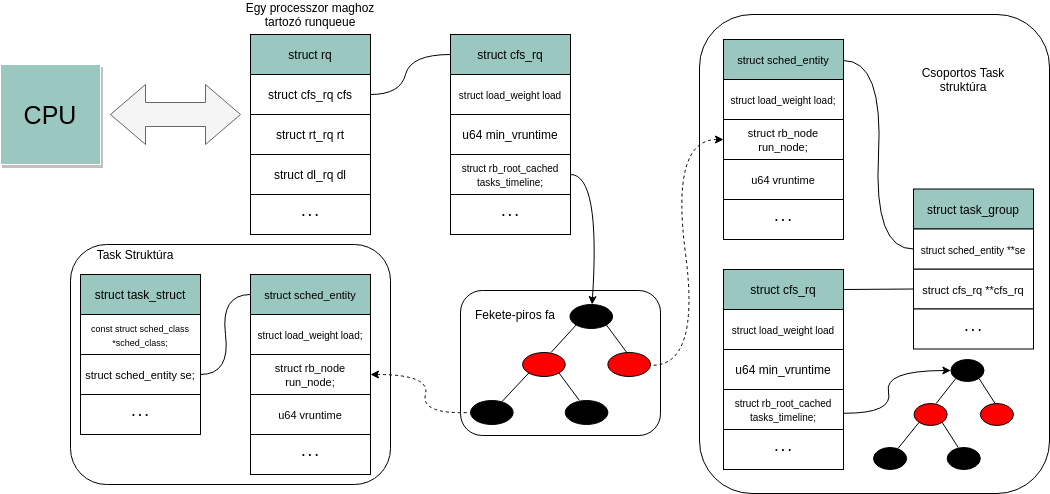
\includegraphics[width=\textwidth]{images/structureHierarchy.png}
\caption{Struktúra hierarchia}
\label{fig:structurehierarchi}
\end{figure}

\Section{Kernel modulok}

Egy modul gyakorlatilag instrukciók sorozata, amit igény szerint, ki- és be lehet tölteni a kernel-be. Kibővíti a kernel funkcionalitását, anélkül hogy újra kelljen indítani a rendszert. Minden magasabb szintű kernel komponenst (mint például fájlrendszerek, I/O eszköz driver, hálózati rétegek) meg lehet írni modulként, és be lehet tölteni a kernel-be \cite{salzman2007linux, bovet2005understanding}.

Az éppen aktuálisan betöltött moduljainkat, le tudjuk kérdezni az \texttt{lsmod} paranccsal, ami a \texttt{/proc/modules} fájl tartalmát listázza.

A modulok ELF objektumként tárolódnak a fájlrendszeren, amik a kernelhez vannak linkelve, ezt a linkelést az \texttt{insmod} paranccsal tudjuk elvégezni.
A modulok egy duplán láncolt listában tárolódnak.
Ha ebből a listából el szeretnénk távolítani egy modult (\textit{unlink} művelet), az \texttt{rmmod} programot használhatjuk, ami a következő műveleteket végzi el:
\begin{enumerate}
	\item Beolvassa a parancssorból annak a modulnak a nevét, amit el kívánunk távolítani.
	\item Megnyitja a \texttt{/proc/modules} fájlt és leellenőrzi, hogy a modul, ténylegesen linkelve van-e a listába.
	\item Meghívja a \texttt{delete\_modul()} rendszerhívást és továbbadja neki a modul nevét.
	\item Terminálódik.
\end{enumerate} 

Minden kernel modulnak kell hogy legyen legalább két eljárása, az egyik ilyen az \texttt{init\_module()}.
Ez egy inicializációs eljárás, az \texttt{init\_module()} hívódik meg amikor beszúrjuk a modult az \texttt{insmod} paranccsal.
A másik a \texttt{cleanup\_module()}, ami pedig az eltávolítás során (\texttt{rmmod}) hívódik meg.
A 2.3.13.-as kernel verzióban bevezettek egy újítást, ami szerint, mi határozhatjuk meg az eljárások neveit. Ehhez használjuk a \texttt{module\_init()} és a \texttt{module\_exit()} makrókat. Tipikusan, az \texttt{init\_module()}-ban írjuk meg a programunkat, ami lehet hogy kicserél egy kernel függvényt a miénkre vagy regisztrál valamilyen kezelőt a kernel-hez. A \texttt{cleanup\_module()}-nak pedig az lenne a feladata, hogy visszavonja a módosításokat, amit az \texttt{init\_module()} elvégzett.
%TODO referencia: https://www.kernel.org/doc/htmldocs/kernel-hacking/routines-init-again.html

A \texttt{printk()} függvénynek, nem a felhasználóval történő kommunikáció a fő szerepe (annak ellenére, hogy az aktuálisan ilyen célból került felhasználásra). Ez egy naplózási eszköz (log) a kernel számára, amivel valamilyen fontos információt vagy hibaüzenetet továbbít. Az üzeneteknek, különböző fontossági szintjük van. Ezeket a szinteket hívjuk \texttt{console\_loglevel}-nek, ami egy kernelbeli változó, aminek a szintjeit 0-7-ig a következőket jelentik. 

%TODO referencia: https://www.kernel.org/doc/html/latest/core-api/printk-basics.html
\begin{enumerate}
\setcounter{enumi}{-1}
	\item KERN\_EMERG \- A rendszerünk már használhatatlan állapotba került.
	\item KERN\_ALERT \- Problémák adódtak, amelyek megoldásáról gondoskodnunk kell.
	\item KERN\_CRIT \- Kritikus események jelentkeztek.
	\item KERN\_ERR \- Nem kritikus hibák jelzése.
	\item KERN\_WARNING	\- Figyelmeztetések, amikre oda kell figyeljünk.
	\item KERN\_NOTICE \- Normális, általános események
	\item KERN\_INFO \- Információ továbbítás ami nem igényel beavatkozást.
	\item KERN\_DEBUG \- Kernelbeli hibakiíratás, egy kimenet a kernel oldalról, hogyha a fejlesztő bekapcsolta a \texttt{debugging at compile time}-ot.
\end{enumerate}
Az aktuális console\_loglevel-t, meg tudjuk jeleníteni futásidőben, a következő paranccsal:
\begin{cpp}
$ cat /proc/sys/kernel/printk 
4        4        1        7
\end{cpp}
%$
Ezek a számok, az aktuális, alapértelmezett, minimális és boot-time-default log szinteket mutatják.

A kernel modulok fejlesztése, az azzal kapcsolatos tudnivalók a dolgozat szempontjából azért lényegesek, mert ezek segítségével lehet hatékony és elegáns hozzáférést biztosítani az ütemezőhöz.
A későbbiekben majd látni fogjuk, hogy egy saját fejlesztésű kernel modul segítségével hogyan tudunk az ütemezésre vonatkozó fontos információkat kinyerni a kernelből.

\Section{Rendszert hangoló szolgáltatások}

\SubSection{Tuned}
Tuned egy rendszer hangoló szolgáltatás amely elérhető GNU/Linux-on.
A tuned program segítségével, a következő feladatokat végezhetjük el.
\begin{itemize}
\item Megfigyelhetjük vele a csatlakoztatott eszközöket, az udev eszközkezelő felhasználásával.
\item Hangolhatunk a rendszerbeállításainkon, kiválasztott profilok szerint.
\item Plug-in alapú architektúrájanak köszönhetően, különböző típusú konfigurációs beállításokat módosíthatunk mint például sysctl, sysfs és kernel boot paraméterek.
\item Támogatja az eszközök gyors csatlakoztatását, és vezérelhető parancssorból vagy a D-Bus-on keresztül, így könnyen integrálhatjuk a meglévő adminisztrációs megoldásokba: például a Cockpit.
\end{itemize}

A tuned általánosan egy daemon szolgáltatásként működik, azonban létezik egy egyszerű processzként futtatható változata is, ekkor viszont limitáltabb a funkciókészlete.
A tuned szolgáltatással statikus profilokat alkalmazhatunk, a saját rendszerünkhöz mérten (Készíthetünk saját profilt is).
Ezeket akár cron segítségével cserélgethetjük bizonyos időközönként.
Lehetőségünk van még egy dinamikus hangolási mód kiválasztására is, így a tuned szolgáltatás 10 másodpercenként újrahangolja a rendszert.

\SubSection{Tuna}

A tuna egy olyan eszköz, amellyel szabályozhatjuk az egyes ütemezési politikákat, valós idejű prioritásokat és a processzor affinitást. 
A felhasználók valós időben láthatják, a módosításaik eredményét.
A tuna programmal lehetőségünk van processzor magok izolációjára, az izolált processzor magokhoz pedig rendelhetünk folyamatokat.
Grafikus felhasználói felülettel rendelkezik amivel akár megfigyelhetjük a processzor topológiát, ez hasznos lehet problémák kiszűrése esetén.
Folyamatok hangolása a tradicionális GNU/Linux eszközökkel egyesek szerint ijesztő és bonyolult lehet, nekik ajánlott a tuna program használata. A tuna lecsökkenti a komplexitást és egy stabil eszközt biztosít számukra is, amelyet kezelhetnek parancssorból vagy a grafikus felhasználói felület használatával.

